\documentclass{article}
\usepackage{graphicx} % Required for inserting images
\usepackage{float}    % For forcing figure positions
\usepackage{framed}   % For adding frames around images
\usepackage{listings} % For Java code examples
\usepackage{booktabs}  % For better table formatting
\usepackage{hyperref}
\usepackage{tikz}
\usetikzlibrary{trees}

\title{Introduction to Spring Framework}
\author{Lahfari Bilal}
\date{\today}

% Settings for Java code formatting
\lstset{ 
    language=Java,
    frame=single,
    basicstyle=\ttfamily,
    numbers=left,
    numberstyle=\tiny,
    breaklines=true,
    showstringspaces=false,
    captionpos=b,
    xleftmargin=\parindent,
    framexleftmargin=10pt,
    framexrightmargin=10pt,
    framextopmargin=5pt,
    framexbottommargin=5pt
}

\begin{document}

\maketitle

\section{Spring framework}
\subsection{What is Spring framework?}

The \textbf{Spring Framework} is an open-source framework designed for building enterprise-level applications in Java. It simplifies the development process by providing a comprehensive programming and configuration model, making it easier to create robust and scalable applications.

\begin{figure}[H]
    \centering
    \begin{framed}
        
\includegraphics[width=0.8\linewidth]{images/spring_logo.png}
    \end{framed}
    \caption{Spring framework}
    \label{fig:spring-logo}
\end{figure}

\subsection{Spring core concepts}

\subsubsection{Inversion of Control (IoC) concept}

\textbf{Inversion of Control} is a design principle where the control over object creation and management is transferred from the application code to a container or framework—in this case, \textbf{the Spring IoC container}. This means that instead of objects creating their dependencies, the IoC container manages their lifecycle and dependencies. This leads to more modular and maintainable code, as components can be easily replaced or modified without affecting other parts of the application.

\begin{figure}[H]
    \centering
    \begin{framed}
        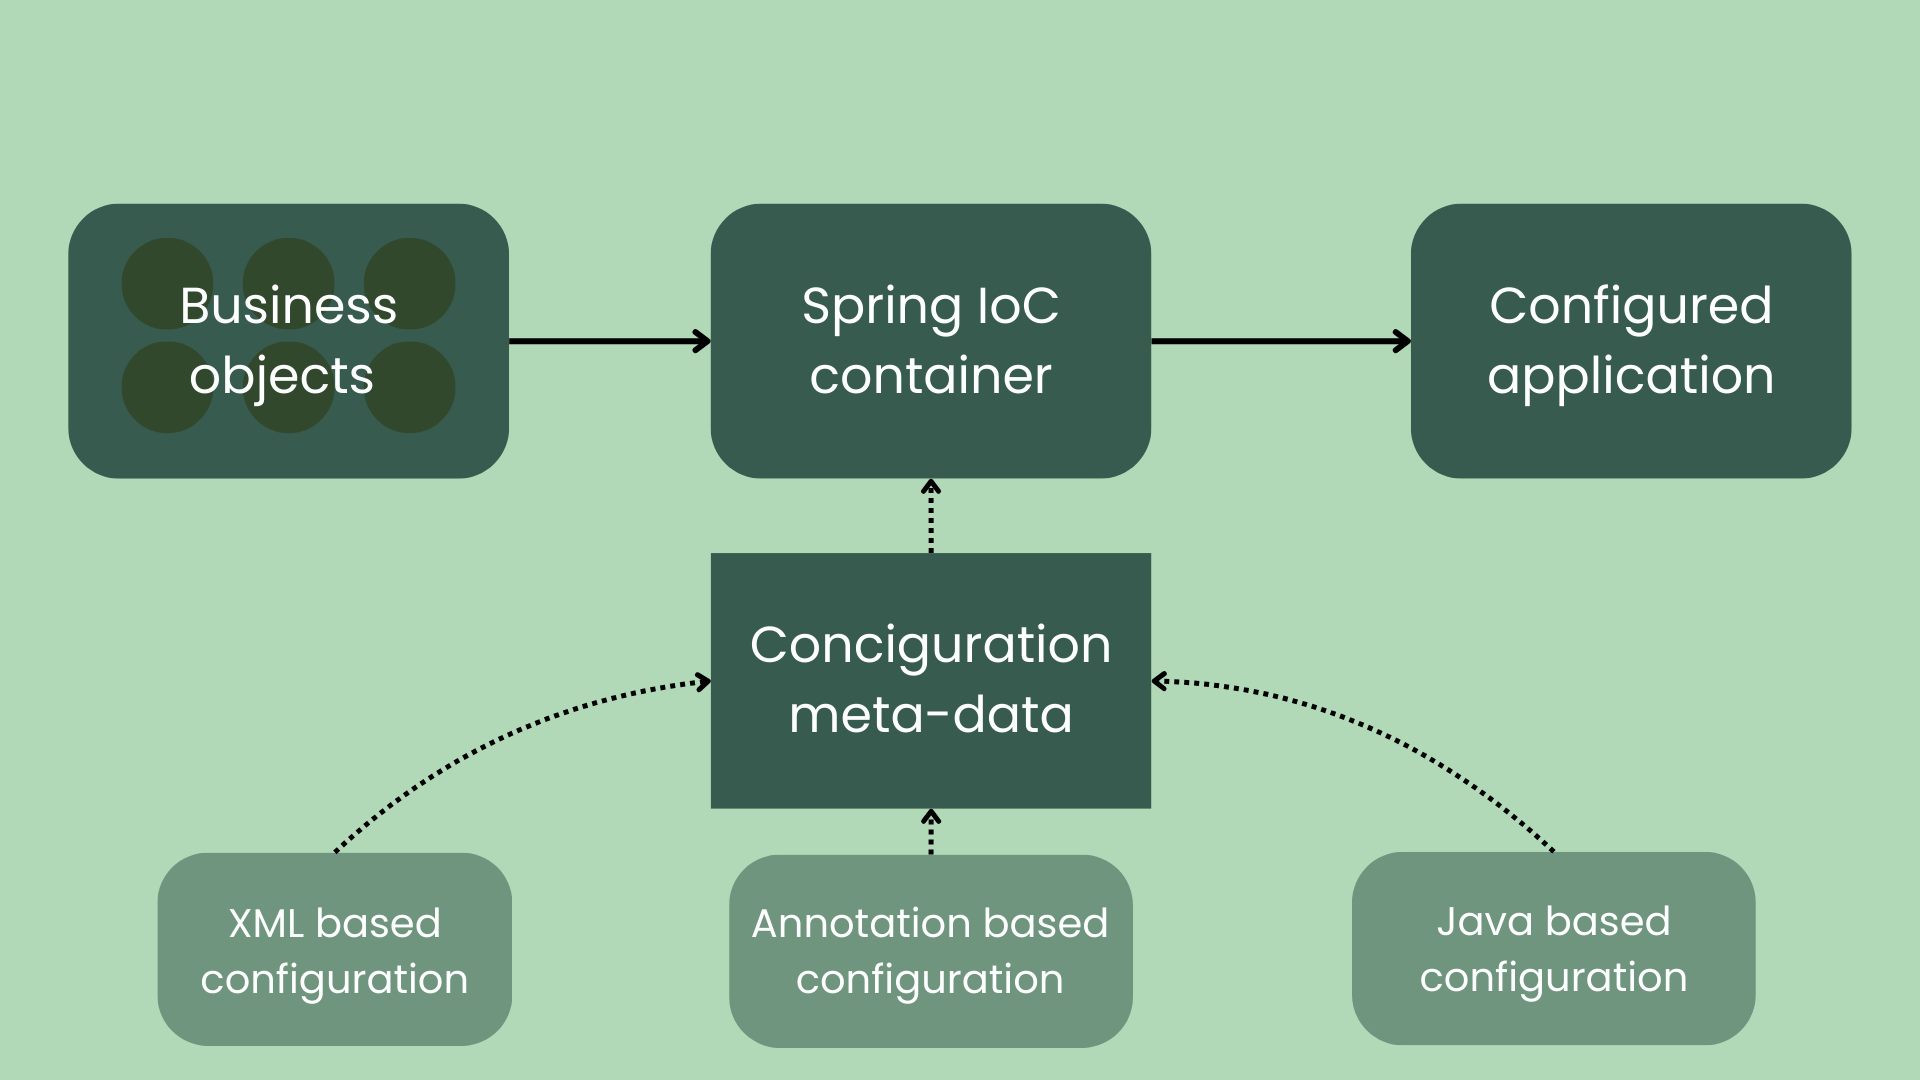
\includegraphics[width=0.9\linewidth]{images/sspring_ioc_container.png}
    \end{framed}
    \caption{Spring IoC container concept}
    \label{fig:spring-ioc-container}
\end{figure}

\subsubsection{IoC Example}

To demonstrate Inversion of Control, here’s a Java code example showing a simple Spring configuration:



\begin{itemize}
    \item \textbf{Business objects}: POJO stands for Plain Old Java Object. These are basic Java classes that represent the business logic or data for your application. They don’t have any specific Spring code in them—they’re just simple Java objects that define your data and operations.

    \item \textbf{Spring IoC container}: The IoC (Inversion of Control) Container is the central part of Spring. It’s responsible for creating, managing, and assembling your objects (the POJOs) and their dependencies.
    
    \item \textbf{Configuration metadata}: The Configuration Metadata is where you define the settings or instructions for the IoC container. It tells the container what objects (beans) to create and how they should be wired together.
    
    \begin{itemize}
        \item \textbf{XML-based}: You write XML files to specify which beans (objects) to create and how they’re connected.
        \item \textbf{Annotation based}: You use Java annotations directly in your code to tell Spring which classes to use and how to connect them.
        \item \textbf{Java-based}: You use Java code to configure the beans and dependencies, typically through \texttt{@Configuration} classes.
    \end{itemize}
    
    \item \textbf{Application}: Once the IoC container reads the configuration metadata and assembles the beans (POJOs), it results in a fully configured application.
\end{itemize}

\subsubsection{Spring beans and dependency injection}
\begin{itemize}
    \item \textbf{Spring Beans} 
    A Spring bean is an object that is instantiated, assembled, and managed by the Spring IoC container. These beans represent the backbone of a Spring application, encapsulating the application's logic and functionality. The management of beans includes their lifecycle, configuration, and dependencies, which are defined through metadata provided by the developer.

    \item \textbf{Dependency injection} : is a design pattern used to implement IoC. It allows the Spring container to provide an object’s dependencies rather than having the object create them itself. This leads to loose coupling between components and enhances testability.

\begin{figure}[H]
    \centering
    \begin{framed}
        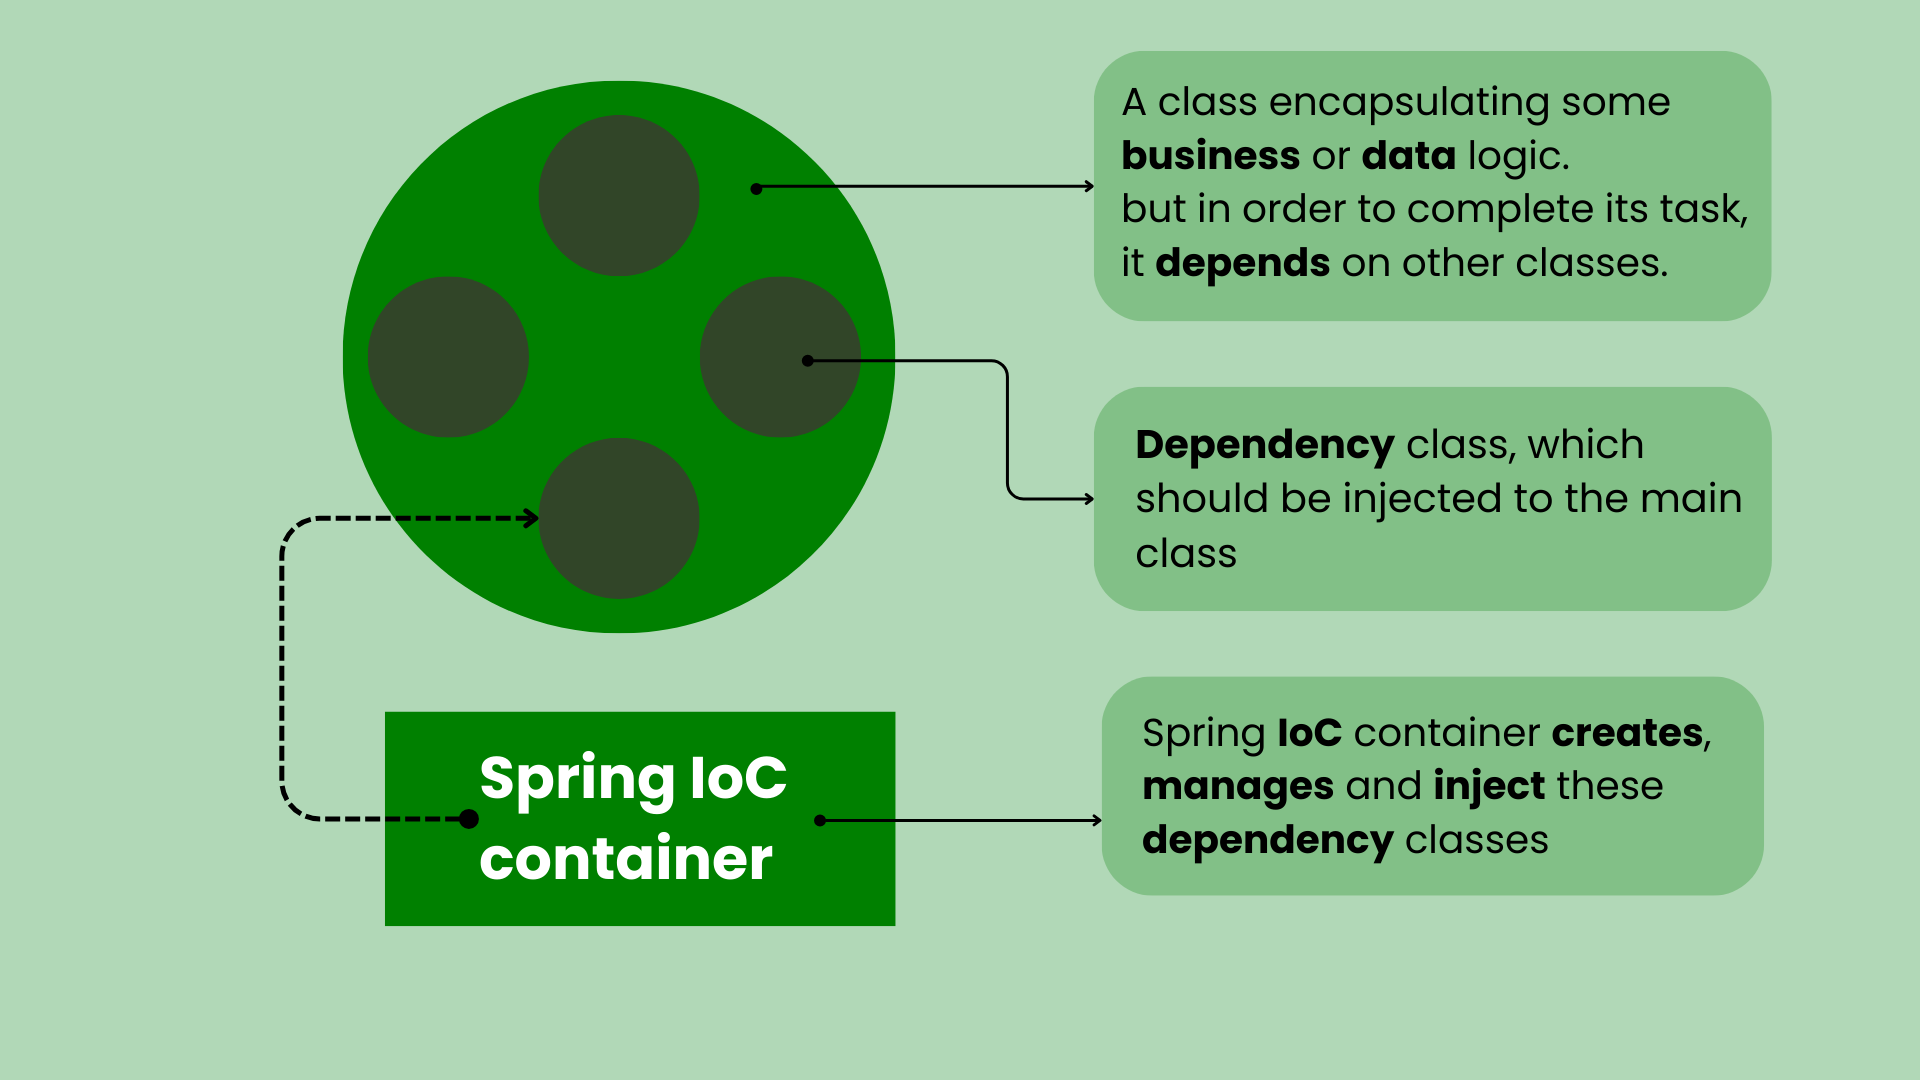
\includegraphics[width=0.9\linewidth]{images/dependency_injection.png}
    \end{framed}
    \caption{Dependency injection of beans}
    \label{fig:spring-ioc-container}
\end{figure}
    

\end{itemize}




\subsubsection{Dependency Injection Examples}
\begin{enumerate} 
    \item \textbf{XML based configuration}\label{sec:ioc-xml-config}
    
    \item \textbf{Annotation based configuration}\label{sec:ioc-annotation-config}

    \item \textbf{Java based configuration}\label{sec:ioc-java-config}
\end{enumerate}
    
\section{Spring boot}

\textbf{Spring Boot} is an extension of the Spring Framework that simplifies the process of developing Spring applications. For beginners, understanding how Spring Boot relates to the Spring Framework can help clarify its purpose and advantages.

\begin{figure}[H]
    \centering
    \begin{framed}
        
\includegraphics[width=0.8\linewidth]{images/spring_boot_logo.png}
    \end{framed}
    \caption{Spring boot}
\end{figure}

\subsection{Key features of Spring boot} 
\begin{itemize}
    \item \textbf{Auto-Configuration} : Spring Boot automatically configures your application based on the libraries you include. For example, if you add a library for web development, it will set up a web server for you without needing extensive configuration.

    \item \textbf{Standalone applications} : 
    With Spring Boot, you can create standalone applications that run independently. It includes an embedded web server (like Tomcat), so you don’t need to deploy your application to an external server.

    \item \textbf{Starter dependencies} : Instead of manually specifying each dependency in your project configuration file, Spring Boot provides \texttt{starters} that bundle commonly used libraries together. For example, spring-boot-starter-web includes everything needed for a web application.

\end{itemize}



\section{Setting up a Spring boot application} 

\subsection{Prerequisites} 

\subsubsection{Java development kit (JDK) }
You need to have Java installed on your system. Spring Boot 3.x requires at least \textbf{Java 17 or higher} Ensure that your Java version is compatible with the Spring Boot version you plan to use.

\subsubsection{Build tools} 
You need a build tool to manage your project dependencies and build processes. The two most common build tools used with Spring Boot are : 
\begin{itemize}
    \item \textbf{Maven} : Version 3.6.3 or later is required.
    \item \textbf{Gradle} : Versions 7.x (7.5 or later) and 8.x are supported
\end{itemize}


\subsubsection{Integrated development environment (IDE)} 
\begin{itemize}
    \item \textbf{Eclipse IDE}
    \item \textbf{Intellij IDEA}
    \item \textbf{Visual studio code}
\end{itemize}


\subsection{Creating Our First Project}
\subsubsection{Bootstrapping the project}

It is recommended to use Spring Initializr (\href{https://start.spring.io/}{https://start.spring.io/}) to set up a Spring Boot project due to the following reasons:
\begin{itemize}
    \item Quickly generates project structure and dependencies.
    \item Allows selection of required modules (e.g., Spring Web, Spring Data JPA).
    \item Provides pre-configured Maven/Gradle builds.
    \item Saves time and simplifies the setup process.
\end{itemize}

\begin{figure}[H]
    \centering
    \begin{framed}
        
\includegraphics[width=0.6\linewidth]{images/spring_init.png}
    \end{framed}
    \caption{Spring initializr}
    \label{fig:spring-ioc-container}
\end{figure}




\subsubsection {Project strcuture}

\begin{tikzpicture}

 \tikzset{
    level 1/.style={sibling distance=50mm},
    level 2/.style={sibling distance=40mm},
    level 3/.style={sibling distance=30mm},
    level 4/.style={sibling distance=20mm},
    level 5/.style={sibling distance=10},
  }
  
  \node {MySpringBootProject} 
    child { node {src} 
      child { node {main} 
        child { node {java} 
          child { node {com} 
            child { node {example} 
              child { node {demo} 
                child { node {DemoApplication.java} }
              }
            }
          }
        }
        child { node {resources} 
          child { node {application.properties} }
        }
      }
      child { node {test} 
        child { node {java} 
          child { node {com} 
            child { node {example} 
              child { node {demo} 
                child { node {DemoApplicationTests.java} }
              }
            }
          }
        }
      }
    }
    child { node {pom.xml} };
\end{tikzpicture}

\begin{enumerate}
    \item \textbf{src/main/java}: 
    \begin{itemize}
        \item This directory contains the main source code for your application.
        \item It is organized by package, typically following the reverse domain name convention (e.g., \texttt{com.example.yourapplication}).
        \item The main class (e.g., \texttt{YourApplication.java}) contains the \texttt{main} method that starts the Spring Boot application.
    \end{itemize}

    \item \textbf{src/main/resources}:
    \begin{itemize}
        \item This folder is for resource files that your application needs, such as configuration files and static assets.
        \begin{itemize}
            \item \texttt{static}: Contains static files like CSS, JavaScript, and images that can be served directly.
            \item \texttt{templates}: Contains server-side templates (e.g., Thymeleaf or FreeMarker) used for rendering dynamic web pages.
            \item \texttt{application.properties}: A key configuration file where you define various settings for your application, such as server port, database connection details, and other properties.
        \end{itemize}
    \end{itemize}

    \item \textbf{src/test/java}:
    \begin{itemize}
        \item This directory is for test classes that correspond to your main application code.
        \item It follows the same package structure as \texttt{src/main/java}, allowing you to keep tests organized alongside the code they test (e.g., \texttt{YourApplicationTests.java}).
    \end{itemize}



    \item \textbf{pom.xml}:
    \begin{itemize}
        \item This is the Maven build file that manages project dependencies, plugins, and other configurations.
        \item It specifies the Spring Boot starter dependencies you are using (like \texttt{spring-boot-starter-web} for web applications) and other libraries necessary for your project.
    \end{itemize}


\end{enumerate}


\section{Conclusion}

The Spring Framework and Spring Boot provide powerful tools for building scalable and maintainable enterprise-level applications. By leveraging concepts like Inversion of Control (IoC) and Dependency Injection, developers can create modular, testable, and easily configurable systems. Spring Boot further simplifies the development process by offering auto-configuration, standalone applications, and pre-configured dependencies, making it an ideal choice for modern Java-based applications. Understanding the key features and setup process of both Spring and Spring Boot will help developers streamline their application development and improve productivity.





\end{document}
